\documentclass[tikz,border=3pt]{standalone}
\usetikzlibrary{positioning,arrows.meta,shapes.geometric,backgrounds}

\begin{document}

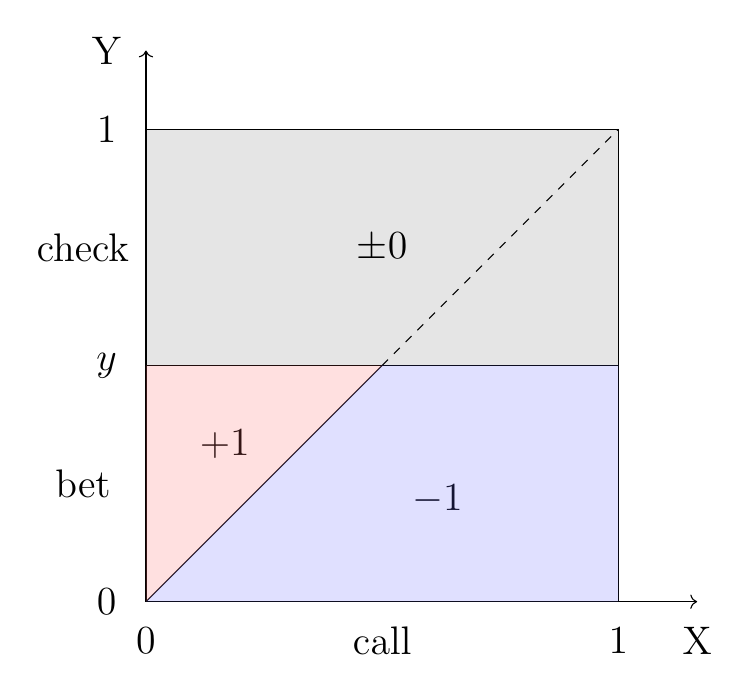
\begin{tikzpicture}

\draw[->] (0,0) --(0,7);
\draw[->] (0,0) --(7,0);
\draw (0,6) --(6,6) --(6,0);
\draw (0,3) --(6,3);
\draw (0,0) --(3,3);
\draw[dashed] (3,3) --(6,6);

\node[font=\Large] at (7,-0.5) {X};
\node[font=\Large] at (-0.5,7) {Y};

\node[font=\Large] at (0,-0.5) {$0$};
\node[font=\Large] at (6,-0.5) {$1$};
\node[font=\Large] at (-0.5,0) {$0$};
\node[font=\Large] at (-0.5,6) {$1$};

\node[font=\Large] at (-0.5,3) {$y$};

\node[font=\Large] at (3,4.5) {$\pm 0$};
\node[font=\Large] at (3.7,1.3) {$-1$};
\node[font=\Large] at (1,2) {$+1$};

%% 範囲説明
% X axis
\node[font=\Large] at (3,-0.5) {call};
% Y axis
\node[font=\Large] at (-0.8,4.5) {check};
\node[font=\Large] at (-0.8,1.5) {bet};

\fill[black, opacity=0.1] (0,3) rectangle (6,6);
\fill[red!60, opacity=0.2] (0,0) --(3,3) --(0,3) --cycle;
\fill[blue!60, opacity=0.2] (0,0) --(6,0) --(6,3) --(3,3) --cycle;

\end{tikzpicture}
\end{document}
